\chapter{Results}
\label{ch:results}

This chapter has two parts.
Section~\ref{sec:pilot-results} reports the fifteen-epoch pilot runs
that fixed the design (Section~\ref{sec:pilots}); their numbers are
correct records of what happened but their seeds, platforms and lengths
are those of pilots, and no claim of the thesis rests on them alone.
Section~\ref{sec:grid-results} reports the final grid against the
hypotheses of Section~\ref{sec:hypotheses}.

\section{Pilot runs}
\label{sec:pilot-results}

\subsection{Executed runs}
\label{sec:executed-fixed}

\subsubsection{Test A, whitened (\texttt{advantage\_norm=whiten})}

Config: \path{configs/cpr_testA_always2.json}.
Partner: frozen always-2.
Folders: \path{checkpoints/cpr_log_testA_always2} (run) and
\path{checkpoints/cpr_log_testA_a0} (same Test~A with opening A0
logged --- the A0 photograph).

Outcomes:
\begin{itemize}
\item Opening-step critic: raw A0 \(\mathbf{+39.8}\) on 1 versus
  \(\mathbf{+6.2}\) on 2.
\item After batch whitening, A0 \(\mathbf{+1.38}\) versus
  \(\mathbf{+0.75}\).
\item Policy still peaked on 2.
  Take-1 live-step \(\mathbf{6\% \to 3\%}\).
  Survival \(\mathbf{28/225}\).
\item Open-1 share: about \(\mathbf{27\%}\) floor, falling
  (epoch \(1 \to 15\)).
\item Take-1 live-step at epoch 15: \(\mathbf{3\%}\).
\end{itemize}

Read \textbf{openings}, not only live-step mix: after a first 1,
\(R\colon 8\to 9\) and \((2,2)\) is a fixed point, so a surviving policy
can be mostly 2s on the tape while every game opened 1.

\subsubsection{Test B, whitened}

Config: \texttt{configs/cpr\_testB\_always1.json}.
Partner: frozen always-1.
Opening A0 also logged (\texttt{testB\_a0}).

Outcomes: survival \(\mathbf{219/225}\); opening 1 and opening 2 received
the same star; mix \(\mathbf{80\% \to 38\%}\) on 2,
\(\mathbf{18\% \to 62\%}\) on 3.

Versus a dove, constant-2 pays 72 and lives; constant-1 pays 36.
There is no 64-versus-7 basin that would force copy-1.

\subsubsection{Test A, centered (\texttt{advantage\_norm=center})}

Config: \texttt{configs/cpr\_testA\_center.json}.
Same seed family as whitened Test~A.
Mean-subtract, no \texttt{/std}.
Folder: \texttt{checkpoints/cpr\_log\_testA\_center}.
15 epochs, frozen always-2.

Table~\ref{tab:whiten-vs-center} is the whitened-versus-centre contrast on
that seed family.

\begin{table}[ht]
\centering
\small
\caption{Test~A outcomes under batch whitening versus centre-only
  advantages (same seed family, frozen always-2).
  Open-1 share is the primary readout; live-step take-1 is not.}
\label{tab:whiten-vs-center}
\begin{tabularx}{\textwidth}{>{\raggedright\arraybackslash}p{3.4cm}XX}
\toprule
 & Whitened Test A & Center Test A \\
\midrule
Take-1 live-step, epoch 15 & 3\% & 9\% \\
Open-1 share, epoch \(1 \to 15\) &
  \(\sim 27\%\) floor, falling &
  \(\mathbf{27\% \to 87\%}\) (100\% at epoch 12) \\
Survival & 28/225 &
  epoch 1: 2/15; epoch 12: \(\mathbf{15/15}\); epoch 15: 13/15 \\
Open-1 A0 (what PPO saw) & +1.38 whitened &
  \(\mathbf{+16.7}\) centered (raw still \(\sim +40\)) \\
Open-2 A0 & +0.75 & \(\mathbf{-5.7}\) \\
\bottomrule
\end{tabularx}
\end{table}

Later 2s still have large \emph{raw} GAE (smear).
After centering they sit near 0; openings of 1 do not.

Run extras: take-3 live-step \(\mathbf{8.5\% \to 0\%}\); survival
\(\mathbf{134/225}\); last three epochs \(\mathbf{41/45}\) openings were
1.

\subsubsection{Test B, centered}

Config: \path{configs/cpr_testB_center.json}.
Folder: \path{checkpoints/cpr_log_testB_center}.
Frozen always-1, seed 0.

Outcomes: survival \(\mathbf{223/225}\); live mix \(\mathbf{98\%}\) on 2;
open-1 share \(\mathbf{13\% \to 13\%}\) (2/15 last epoch).
Did not copy-1.
Opening A0 on 1 and 2 both large and similar (centred \(\sim +20\) /
\(+22\)).

\subsubsection{Test A center, extra seeds}

Folder: \texttt{checkpoints/cpr\_log\_testA\_center\_s12}
(\texttt{exp1\_} seed 1, \texttt{exp2\_} seed 2).

\begin{itemize}
\item Seed 1: open-1 \(\mathbf{27\% \to 93\%}\), survival
  \(\mathbf{113/225}\), last epoch 14/15 opened 1.
\item Seed 2: open-1 \(\mathbf{27\% \to 7\%}\), survival
  \(\mathbf{160/225}\), last epoch \(\mathbf{14/15}\) opened 0.
\end{itemize}

Same center flag, same frozen hawk.
Heterogeneity is a recorded outcome, not a claim.
These extra seeds are the pre-fix family (shared sampling stream;
Chapter~\ref{ch:method}).

\subsubsection{Seed-fixed Test A, centre and whitened (8--9 Sep, all L40S)}

After the trainer reseed fix.
Configs \path{configs/cpr_testA_center.json} and
\path{configs/legacy/cpr_testA_always2.json}.
Folders \path{checkpoints/cpr_log_testA_center_reseed} and
\path{checkpoints/cpr_log_testA_whiten_reseed}, three seeds \(\times\) 15
epochs; plus whitened seed~0 for 30 epochs
(\path{checkpoints/cpr_log_testA_whiten_reseed_e30}).

Identity of agent-1 openings in epochs 1--5: centre pairs \(0.56\)--\(0.61\),
whitened pairs \(0.63\) (pre-fix whitened \(s1\) vs \(s2\) was \(1.00\)).
Outcomes are in Chapter~\ref{ch:results}.
Table shorthand (last-open, last surv, last ret, leave-2 last3, first
majority) is defined at the start of this chapter: last-open is the 15
first-round harvests of epoch 15, not a count of epochs.
Do not call epoch 15 an endpoint: the 30-epoch whitened seed~0 is the
continuation of the 15-epoch snapshot.

Figure~\ref{fig:openings} plots the first-to-last open-1 share for
whitened Test~A and the three centred seeds, using only those endpoint
numbers.

\begin{figure}[ht]
\centering
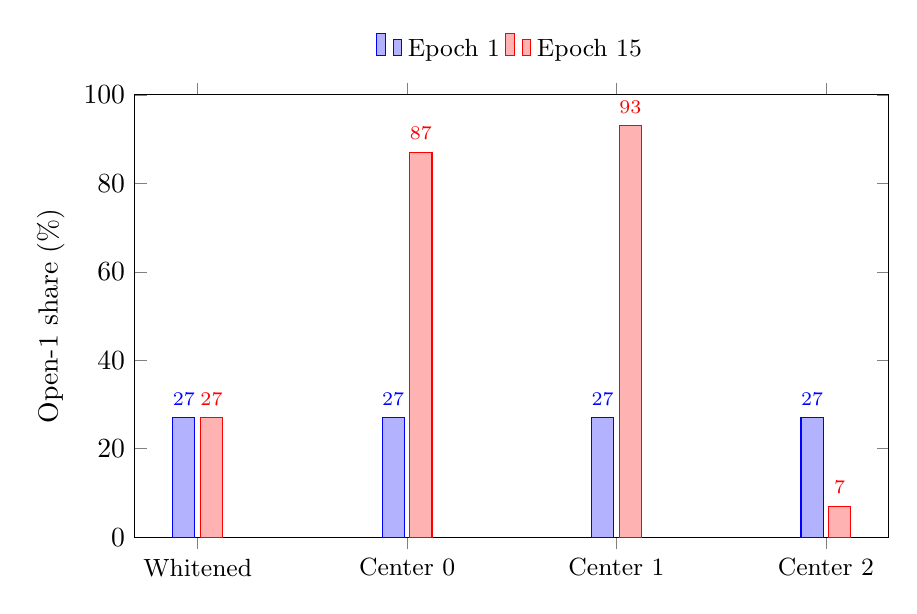
\begin{tikzpicture}
\begin{axis}[
  ybar,
  bar width=8pt,
  width=0.92\textwidth,
  height=7.2cm,
  ylabel={Open-1 share (\%)},
  ymin=0, ymax=100,
  symbolic x coords={Whitened, Center 0, Center 1, Center 2},
  xtick=data,
  xticklabel style={font=\small},
  legend style={at={(0.5,1.05)}, anchor=south, legend columns=2,
    font=\small, draw=none},
  nodes near coords,
  nodes near coords style={font=\scriptsize, /pgf/number format/fixed},
  every node near coord/.append style={yshift=1pt},
]
\addplot coordinates {(Whitened,27) (Center 0,27) (Center 1,27) (Center 2,27)};
\addplot coordinates {(Whitened,27) (Center 0,87) (Center 1,93) (Center 2,7)};
\legend{Epoch 1, Epoch 15}
\end{axis}
\end{tikzpicture}
\caption{Test~A open-1 share at the first and last epoch against a frozen
  hawk.
  Whitened last-epoch share is not recorded as a separate number; the
  executed note is a \(\sim 27\%\) floor, falling, so the last bar repeats
  that floor rather than inventing a lower point.
  Centre seeds~0 and~1 rise to \(87\%\) and \(93\%\).
  Centre seed~2 falls to \(7\%\) (last epoch almost all opening~0, not~1).
  Survival: whitened \(28/225\); seeds \(0/1/2\): \(134/225\),
  \(113/225\), \(160/225\).}
\label{fig:openings}
\end{figure}

\subsection{Executed runs --- two learners}
\label{sec:executed-two}

Same lock, \texttt{advantage\_norm=center}, entropy 0.05.
Claim statistic: share of episodes that do \textbf{not} open 2.
Do not put unmatched epoch lengths in one versus-naive table.

\subsubsection{Centred naive--naive, 15 epochs, seeds 0--2}

Config \path{configs/cpr_naive_naive_center.json}.
Folders \path{checkpoints/cpr_log_naive_naive_center} (seed 0) and
\path{checkpoints/cpr_log_naive_naive_center_s12} (seeds 1--2).

\begin{table}[ht]
\centering
\small
\caption{Centred naive--naive, 15 epochs.
  Who leaves opening 2 swaps across seeds.
  Live mix at epoch 15 is still mostly 2s on the tape.}
\label{tab:nn}
\begin{tabular}{llll}
\toprule
 & Seed 0 & Seed 1 & Seed 2 \\
\midrule
Surv e1 / e15 & 2/15 / 15/15 & 2/15 / 13/15 & 2/15 / 14/15 \\
Survived & 119/225 & 98/225 & 115/225 \\
A1 last openings & \(15\times 0\) & \(9\times 1\), \(5\times 2\), \(1\times 3\) &
  \(1\times 0\), \(8\times 1\), \(6\times 2\) \\
A2 last openings & \(3\times 1\), \(12\times 2\) &
  \(1\times 0\), \(14\times 1\) & \(13\times 1\), \(2\times 2\) \\
A1 leave-2 first3\(\to\)last3 & \(11\%\to 96\%\) & \(7\%\to 53\%\) &
  \(7\%\to 64\%\) \\
A2 leave-2 first3\(\to\)last3 & \(11\%\to 29\%\) & \(16\%\to 84\%\) &
  \(20\%\to 84\%\) \\
\bottomrule
\end{tabular}
\end{table}

\subsubsection{Centred naive--shaper, three seeds by 15 epochs}

Config \path{configs/cpr_naive_shaper_center.json}.
Folder \path{checkpoints/cpr_log_naive_shaper_center}.
Agent 2: trial update, LR \(3\times 10^{-7}\), \texttt{cliprange=0.1},
extra trial prompt on.

\begin{table}[ht]
\centering
\small
\caption{Centred naive--shaper, 15 epochs.
  Who leaves 2 did not swap: agent 1 dove, agent 2 hawk on all three seeds.}
\label{tab:ns}
\begin{tabular}{llll}
\toprule
 & Seed 0 & Seed 1 & Seed 2 \\
\midrule
Surv e15 & 13/15 & 9/15 & 13/15 \\
Survived & 113/225 & 120/225 & 100/225 \\
A1 last openings & \(1\times 0\), \(13\times 1\), \(1\times 2\) &
  \(1\times 0\), \(14\times 1\) & \(7\times 0\), \(8\times 1\) \\
A2 last openings & \(14\times 2\), \(1\times 3\) &
  \(2\times 1\), \(9\times 2\), \(4\times 3\) & \(14\times 2\), \(1\times 3\) \\
A1 / A2 leave-2 last3 & \(96\%\) / \(0\%\) & \(93\%\) / \(7\%\) &
  \(87\%\) / \(2\%\) \\
A2 leave-2 whole run & 5\% & 5\% & 4\% \\
\bottomrule
\end{tabular}
\end{table}

\subsubsection{Shaper 50 epochs, seed 0}

Folder \path{checkpoints/cpr_log_naive_shaper_center_e50}.
Compare to naive at epoch 15 only.

Epoch 15: 13/15 survived, agent 1 \(13\times 1\), agent 2 \(14\times 2\).
Epoch 50: 15/15, agent 1 \(15\times 1\), agent 2 \(15\times 2\).
Whole run 572/750.
Agent 2 opened 0 or 1 on 25/750 (3.3\%).
No epoch with agent-2 leave-2 majority.

\subsubsection{Info-off shaper, three seeds by 15 epochs}

Config \path{configs/cpr_naive_shaper_center_info_off.json}.
Trial update and LR unchanged; \texttt{transmit\_info=false}.

\begin{table}[ht]
\centering
\small
\caption{Centred naive--shaper with \texttt{transmit\_info=false}.
  Who leaves 2 did not swap.
  Agent-2 leave-2 over the whole run is 16--19\% versus 4--5\% with the
  extra prompt.}
\label{tab:infooff}
\begin{tabular}{llll}
\toprule
 & Seed 0 & Seed 1 & Seed 2 \\
\midrule
Surv e15 & 14/15 & 13/15 & 14/15 \\
Survived & 118/225 & 107/225 & 89/225 \\
A1 last openings & \(14\times 0\) & \(1\times 0\), \(14\times 1\) &
  \(14\times 0\), \(1\times 1\) \\
A2 last openings & \(13\times 2\) & \(12\times 2\) & \(12\times 2\) \\
A1 / A2 leave-2 last3 & \(96\%\) / \(18\%\) & \(89\%\) / \(22\%\) &
  \(89\%\) / \(13\%\) \\
A2 leave-2 whole run & 16\% & 19\% & 16\% \\
\bottomrule
\end{tabular}
\end{table}


\subsubsection{Protocol (as executed)}

Four centred configurations, \(\xi\) on, no other change:
Test~A against a frozen hawk, naive--naive, naive--shaper, and slow-LR
naive--naive, each three seeds \(\times\) 15 epochs of 15 games.
Advantages are mean-centred.
The batch-whitened variant is not repeated on this arm.
The 6~September packet is the pre-fix family (shared seed-0 action
stream).
The 8--9~September packet repeats naive--shaper \(\xi\) and slow-LR
\(\xi\) after the fix, plus a 50-epoch slow-LR \(\xi\) seed~0; Test~A
\(\xi\) and naive--naive \(\xi\) were not repeated; naive--shaper
\(\xi\) at 50 epochs was not obtained (OOM).
A 30-epoch whitened Test~A (deterministic, not \(\xi\)) is in the
seed-fixed Test~A subsection.
The rules text was left unchanged: it does not state a regeneration
schedule, the stock is reported every round, and the unused prompt
clause \texttt{XI\_GROWTH\_CLAUSE} was not spliced in.

For each seed a table of shape (epochs, games, rounds) is drawn once
from a dedicated seed sequence (\texttt{cpr\_env.make\_noise\_table}),
stored as \texttt{noise\_table.npy}, and loaded by every configuration
on the arm.
The draw at a given (epoch, game, round) is therefore identical across
the four arms for the same seed, and independent of any action taken.
That is a measurement device, not a new algorithm
\cite{piche2025}.

Exact checks live in \texttt{tests/test\_cpr\_xi.py}: mean-one
multiplier; \(\xi=1.0\) bit-identical to Stage~A; constant-pair
invariance under i.i.d.\ tables; absorbing zero.

Folders (pre-fix):
\path{checkpoints/cpr_log_testA_center_xi},
\path{checkpoints/cpr_log_naive_naive_center_xi},
\path{checkpoints/cpr_log_naive_shaper_center_xi},
\path{checkpoints/cpr_log_naive_naive_slow2_center_xi}.
Folders (seed-fixed):
\path{checkpoints/cpr_log_naive_shaper_center_xi_reseed},
\path{checkpoints/cpr_log_naive_naive_slow2_center_xi_reseed},
\path{checkpoints/cpr_log_naive_naive_slow2_center_xi_reseed_e50}.
A retired \(\pm 1\)-on-stock Test~A is archived; those numbers are not a
Results table.

\begin{table}[ht]
\centering
\small
\caption{Stage~B GPU, three \emph{nominal} seeds \(\times\) 15 epochs
  (pre-fix, shared action stream).
  Report against Table~\ref{tab:noise-dp}, not only against each other.
  Seed-fixed NS and slow2 are Table~\ref{tab:stageb-reseed}.
  Interpretation is in Chapter~\ref{ch:results}.}
\label{tab:stageb}
\begin{tabular}{lp{3.4cm}p{7.4cm}}
\toprule
Arm & Survived (s0/s1/s2) & Leave-2 last3 \\
\midrule
Test~A \(\xi\) & 119, 41, 93 / 225 &
  98\%, 64\%, 98\%.
  Last openings \(15\times 0\) / \((10\times 1+5\times 2)\) / \(15\times 0\). \\
NN \(\xi\) & 100, 43, 82 / 225 &
  who-doves mixed (seed~2 a2 87\% leave-2; seed~1 both mostly 2) \\
NS \(\xi\) & 90, 71, 75 / 225 &
  a1 96/93/89\%; a2 0/11/11\% hawk \\
slow2 \(\xi\) & 53, 44, 39 / 225 &
  a2 last3 18/18/20\%; last epoch 12--13\(\times 2\) \\
\bottomrule
\end{tabular}
\end{table}

\begin{table}[ht]
\centering
\small
\caption{Stage~B GPU after the trainer reseed fix, three independent
  seeds \(\times\) 15 epochs, all L40S.
  Seed~0 of each arm is the pre-fix seed-0 tape.
  Test~A \(\xi\) and NN \(\xi\) were not repeated.
  Report against Table~\ref{tab:noise-dp}.}
\label{tab:stageb-reseed}
\begin{tabular}{lp{3.4cm}p{7.4cm}}
\toprule
Arm & Survived (s0/s1/s2) & Leave-2 last3 \\
\midrule
NS \(\xi\) reseed & 90, 44, 29 / 225 &
  a1 96/44/33\%; a2 0/22/22\%.
  Last3 surv \(36/45\), \(12/45\), \(5/45\). \\
slow2 \(\xi\) reseed & 53, 61, 34 / 225 &
  a1 69/76/27\%; a2 18/13/22\%.
  Last3 surv \(21/45\), \(24/45\), \(8/45\). \\
slow2 \(\xi\) e50 s0 & 443/750 &
  last-open a1 \(15\times 0\); a2 mixed \(6\times 1+8\times 2+1\times 3\);
  last ret \(70.5/69.2\). \\
\bottomrule
\end{tabular}
\end{table}



These first runs are \textbf{learner versus a frozen constant partner} on the
locked logistic chicken (\(R_0=8\), \(K=40\), \(T=36\),
\texttt{rate\_tenths=9}).
Two-learner numbers follow in Section~\ref{sec:twolearners}; they are not
licensed as ``shaping works.''
Gemma-2-2b-it starts with a strong take-2 prior.
Centre-only advantages (\texttt{advantage\_norm=center}: mean-subtract, no
\texttt{/std}) are the update used in the centred runs.
Default TRL \texttt{masked\_whiten} (batch mean and divide-by-std) is the
whitened contrast.
That difference is an implementation default, not a PPO-paper axiom.

\subsection{What a claim is allowed to use}

Mutual take-2 from \(R=8\) dies around round~4.
A first-step take of \textbf{1} against a take-2 partner moves stock
\(8\to 9\).
At \(R=9\), mutual take-2 is a fixed point and the rest of the horizon can
be farmed.
A first-step take of \textbf{0} against take-2 moves stock \(8\to 11\),
not onto that fixed point.
The opening statistic still counts leave-2 (open 0 or 1).
Those two tokens are not the same basin.

Statistics, decoded for a reader who has not sat the runs
(Chapter~\ref{ch:design} writes the same quantities as
\(\hat{L}\), \(\hat{S}\), \(\hat{G}\)):

\begin{itemize}
\item \textbf{Primary.} Share of episodes that do not open 2 (open 1 or
  open 0). Each epoch is 15 games (5 episodes \(\times\) 3 parallel
  games). The opening is round~1 of each 36-round game.
\item \textbf{Last-open.} The 15 first-round harvests in epoch~15.
  \(10\times 0+5\times 1\) is ten games that opened 0 and five that
  opened 1, not ten epochs.
\item \textbf{Last surv / last ret.} How many of those 15 games reached
  \(T=36\), and the mean learner return on them.
  Stay-on-2 against a hawk is about 7; open-1-then-2s is 71
  deterministic.
\item \textbf{Leave-2 last3.} Leave-2 share over epochs 13--15 (45
  games).
\item \textbf{First majority.} First epoch in which leave-2 exceeded
  \(8/15\).
\item \textbf{Supporting.} Whole-run survival and death round.
\item \textbf{Not the claim.} Live-step action mix.
  After a good opening, a tape of 2s is the \(R=9\) farm.
\end{itemize}

Raw opening advantage already starred that basin.
Under whitening the star was compressed until the prior won on count.

\subsection{Test A --- frozen hawk (always 2)}

\textbf{Whitened.}
Live take-1 fell \(6\%\to 3\%\).
Survival was \(28/225\); deaths around round~4.
Raw opening A0 was about \(+39.8\) on open 1 versus \(+6.2\) on open 2.
After whitening those became \(+1.38\) versus \(+0.75\).
Sign survived; scale did not.

\textbf{Centre-only, seed 0.}
Survival \(134/225\).
Open-1 share \(27\%\to 87\%\); last epoch \(13/15\) opened 1 (from
\(4/15\)).
Epoch 12 was \(15/15\) open 1 and \(15/15\) survived.
Centred opening A0 stayed loud on 1 (\(+16.7\) versus \(-5.7\) on 2; raw on
1 still \(\sim +40\)).
Later 2s in winning games centre near 0: the jackpot stays on the first
step.
Take-3 died (\(8.5\%\to 0\%\)).
Live mix remains mostly take-2 after the opening because that is the
fixed-point farm.

\textbf{Seeds 1 and 2.}
Leaving opening 2 replicates; the restraint \emph{token} need not
(Table~\ref{tab:seeds}).

\begin{table}[ht]
\centering
\caption{Last-epoch openings and run survival for centred Test~A against a
  frozen hawk (pre-fix family, shared sampling stream).
  Seed~2 last epoch is almost all opening~0, not~1.}
\label{tab:seeds}
\begin{tabular}{lll}
\toprule
Seed & Last-epoch openings & Survived \\
\midrule
0 & \(13/15\) opened 1 & \(134/225\) \\
1 & \(14/15\) opened 1 & \(113/225\) \\
2 & \(14/15\) opened 0, one opened 1 & \(160/225\) \\
\bottomrule
\end{tabular}
\end{table}

Seed 2 last epoch left opening 2 via \textbf{0} (\(14/15\)), not 1.
That is leave-2 on the primary statistic.
It is not the \(R=8\to 9\) farm (open 0 vs hawk goes \(8\to 11\)).
Stage~A opening values against a hawk are \(Q(0)=105\) and \(Q(1)=104\),
so both tokens leave 2; the token is not identified by that one-unit gap.

\textbf{Whitened extra seeds (RNG 1--2).}
Seed 0 staying on 2 is not the whole family.
Seed 1 last epoch opened 1 on \(15/15\) (leave-2 last3 \(87\%\), survival
\(97/225\), return \(69.5\)).
Seed 2 last epoch opened 0 on \(12/15\) and 1 on \(3/15\) (leave-2 last3
\(82\%\), survival \(80/225\), return \(69.7\)).
Both extra seeds survived \(15/15\) in the last epoch.

\textbf{Pre-fix family (shared sampling stream).}
Against a frozen hawk, centre-only advantages moved the policy off
opening 2 on three \emph{nominal} seeds.
Batch whitening did that on seeds 1--2 and did not on seed 0
(survival \(28/225\), last epoch \(14\times 2\); that seed-0 tape is MPS).
Treated as a binary leave-2 outcome at three nominal seeds each, the
operators are not distinguishable (whitened \(1/3\) stayed on 2, centred
\(0/3\)).
They differ by the factor \(1/\sigma_{\mathcal{B}}\) in \eqref{eq:norm},
with \(\sigma_{\mathcal{B}}\) measured per update at \(13\)--\(15\)
(Section~\ref{sec:operator}); under Adam that factor is a reweighting of
the policy gradient against the critic, the entropy bonus and the other
batches, not a larger step.
What separates the pre-fix whitened run that stayed on opening 2 from the
five that left it is visible in the opening advantages themselves
(Table~\ref{tab:a0-epochs}): in that MPS seed 0 the post-operator
advantage of opening 2 stayed between \(+0.5\) and \(+1.1\) in every
epoch, because nearly every game in every batch collapsed and there was
no surviving game for the opening-2 games to be compared against, so by
\eqref{eq:logit-update} logit 2 was never pushed down; in whitened seeds
1--2 and in every centred run it turned negative by epoch 4 once
surviving games entered the batches.

\textbf{Seed-fixed Test A, all L40S, \(3\times 15\).}
After the trainer reseed fix the three seeds are independent
(opening identity epochs 1--5 is \(0.56\)--\(0.63\); pre-fix whitened
\(s1\) vs \(s2\) was \(1.00\)).
Centre-only left opening 2 on all three seeds
(Table~\ref{tab:seeds-reseed}): first leave-2 majority at epochs 7, 7, 8;
last-epoch openings \(10\times 0+5\times 1\), \(14\times 0+1\times 1\),
\(14\times 1+1\times 2\); last-epoch survival \(14/15\), \(15/15\),
\(11/15\); last-epoch return \(67.1\), \(80.7\), \(59.1\); leave-2 last3
\(93\%\), \(98\%\), \(91\%\).
Whitened is slower and more seed-variable: leave-2 last3 \(31\%\),
\(96\%\), \(71\%\); first majority at epochs 15, 7, 13; last-epoch
survival \(5/15\), \(13/15\), \(9/15\); last-epoch return \(34.7\),
\(62.4\), \(42.3\); seed 0 last epoch mixed \(8\times 1+7\times 2\).
It is not ``fails to leave'': two of three last epochs have leave-2
majority.

\textbf{Whitened 30 epochs, seed 0.}
Epoch 15 matches the 15-epoch snapshot (survival \(5/15\), return
\(34.7\), leave-2 \(8/15\)).
Leave-2 then stalls through epoch 21 and locks from epoch 23
(\(12/15\) open 1).
Last epoch \(15\times 1\), survival \(13/15\), last3 survival \(42/45\),
return \(64.5\).
Do not call epoch 15 an endpoint.

\textbf{Claim.}
Against a frozen hawk, with independent seeds on the same GPU,
centre-only advantages left opening 2 on three seeds by epoch 8.
Whitening left on a longer and more variable schedule.
The prior yields on the first action when it leaves 2.
It does not become a habit of take-1 across the tape.
Do not write that whitening always keeps the death-open.
Do not treat a 15-epoch last-epoch binary as the operator contrast.
This is a precondition finding: it says whether the prior can leave 2
against a statue that already plays hawk, which operator does so within
the 15-epoch budget used later, and that two-learner runs therefore use
mean-centring.
It is not opponent shaping, and it is not tested off Gemma-2-2b-it on
this lock.

\begin{table}[ht]
\centering
\small
\caption{Opening advantages by epoch for the six Test~A runs against the
  frozen hawk.
  \(k\) is the number of the 15 games that did not open 2;
  \(\tilde{A}(\ne 2)\) and \(\tilde{A}(2)\) are the mean post-operator
  opening advantages of the games that opened 0 or 1 and of the games
  that opened 2 (a dash means no game opened that way).
  Whitened values are in units of the batch standard deviation; centred
  values are in units of return.
  Generated by \texttt{scripts/make\_a0\_table.py} from the
  \texttt{opening\_a0} logs.}
\label{tab:a0-epochs}
\resizebox{\textwidth}{!}{\begin{tabular}{lrrrrrrrrrrrrrrr}
\toprule
 & \multicolumn{3}{c}{Epoch 1} & \multicolumn{3}{c}{Epoch 4} & \multicolumn{3}{c}{Epoch 8} & \multicolumn{3}{c}{Epoch 12} & \multicolumn{3}{c}{Epoch 15} \\
\cmidrule(lr){2-4} \cmidrule(lr){5-7} \cmidrule(lr){8-10} \cmidrule(lr){11-13} \cmidrule(lr){14-16}
Run & $k$ & $\tilde A(\ne 2)$ & $\tilde A(2)$ & $k$ & $\tilde A(\ne 2)$ & $\tilde A(2)$ & $k$ & $\tilde A(\ne 2)$ & $\tilde A(2)$ & $k$ & $\tilde A(\ne 2)$ & $\tilde A(2)$ & $k$ & $\tilde A(\ne 2)$ & $\tilde A(2)$ \\
\midrule
Whitened, seed 0 & 5 & +1.3 & +1.0 & 2 & +1.4 & +0.6 & 3 & +1.3 & +0.6 & 3 & +1.3 & +0.6 & 1 & +1.5 & +1.1 \\
Whitened, seed 1 & 3 & +1.6 & +0.4 & 6 & +1.4 & -0.3 & 10 & +1.2 & -0.3 & 10 & +1.3 & -0.9 & 15 & +1.5 & -- \\
Whitened, seed 2 & 3 & +1.5 & +0.3 & 6 & +1.3 & -0.4 & 5 & +1.3 & -0.4 & 7 & +1.4 & +0.1 & 15 & +1.3 & -- \\
Centred, seed 0 & 5 & +9.2 & +0.8 & 4 & +18.8 & -5.5 & 12 & +17.2 & -16.0 & 15 & +17.6 & -- & 13 & +20.2 & -17.6 \\
Centred, seed 1 & 5 & +9.8 & +1.1 & 9 & +14.3 & -12.2 & 14 & +9.3 & -14.8 & 15 & +13.7 & -- & 14 & +16.1 & -20.5 \\
Centred, seed 2 & 5 & +8.6 & -0.1 & 7 & +17.2 & -15.2 & 14 & +11.4 & -17.3 & 15 & +14.8 & -- & 15 & +17.8 & -- \\
\bottomrule
\end{tabular}
}
\end{table}

\begin{table}[ht]
\centering
\small
\caption{Seed-fixed Test~A against a frozen hawk, all L40S, 15 epochs.
  One learner, not two; the partner is frozen always-2.
  Last-open is the 15 first-round harvests of epoch~15
  (\(10\times 0+5\times 1\) = ten opened 0, five opened 1).
  Last surv / ret are survival and mean return on those 15 games.
  Leave-2 last3 is the leave-2 share over epochs 13--15 (45 games).
  First majority is the first epoch with leave-2 \(>8/15\).
  Identity of openings in epochs 1--5 is \(0.56\)--\(0.63\) between seeds
  (pre-fix whitened \(s1\) vs \(s2\) was \(1.00\)).}
\label{tab:seeds-reseed}
\begin{tabular}{llll}
\toprule
 & s0 & s1 & s2 \\
\midrule
Centre last-open & \(10\times 0,5\times 1\) & \(14\times 0,1\times 1\) & \(14\times 1,1\times 2\) \\
Centre last surv / ret & \(14/15\), \(67.1\) & \(15/15\), \(80.7\) & \(11/15\), \(59.1\) \\
Centre leave-2 last3 & \(93\%\) & \(98\%\) & \(91\%\) \\
Centre first majority & 7 & 7 & 8 \\
Whitened last-open & \(8\times 1,7\times 2\) & \(13\times 1,2\times 0\) & \(7\times 1,3\times 0,5\times 2\) \\
Whitened last surv / ret & \(5/15\), \(34.7\) & \(13/15\), \(62.4\) & \(9/15\), \(42.3\) \\
Whitened leave-2 last3 & \(31\%\) & \(96\%\) & \(71\%\) \\
Whitened first majority & 15 & 7 & 13 \\
\bottomrule
\end{tabular}
\end{table}

\begin{figure}[ht]
\centering
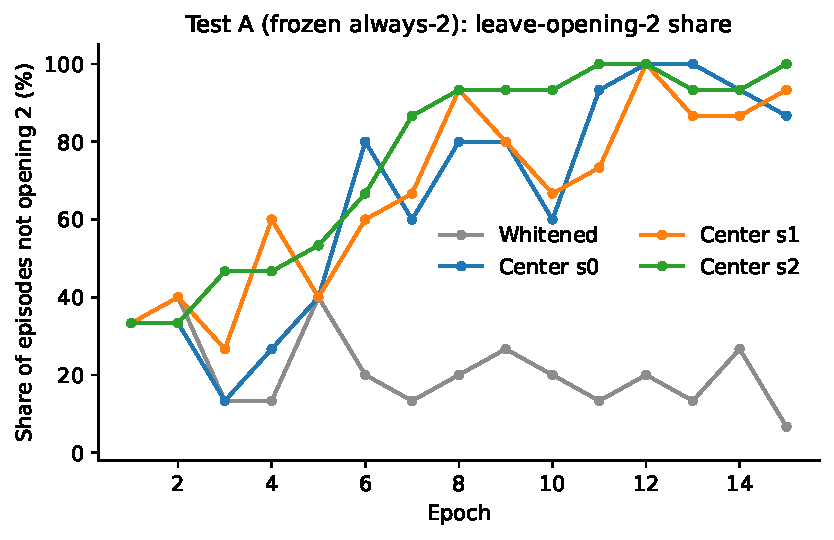
\includegraphics[width=0.92\textwidth]{figures/fig_openings_testA.pdf}
\caption{Share of episodes that do not open 2 (open 0 or 1) against a
  frozen always-2 partner.
  Pre-fix family: the whitened curve is MPS seed~0, which stays on the
  death-open; whitened seeds 1--2 left opening 2 (text).
  Centre-only seeds 0--2 leave opening 2.
  Seed-fixed all-L40S numbers are Table~\ref{tab:seeds-reseed}.
  Seed~2's last epochs leave 2 mostly via opening~0, not 1
  (Table~\ref{tab:seeds}): leave-2, not the \(R=9\) farm.
  This figure is the opening statistic.
  It is not a 36-step dove policy and not a shaping result.}
\label{fig:openingsA}
\end{figure}

\begin{figure}[ht]
\centering
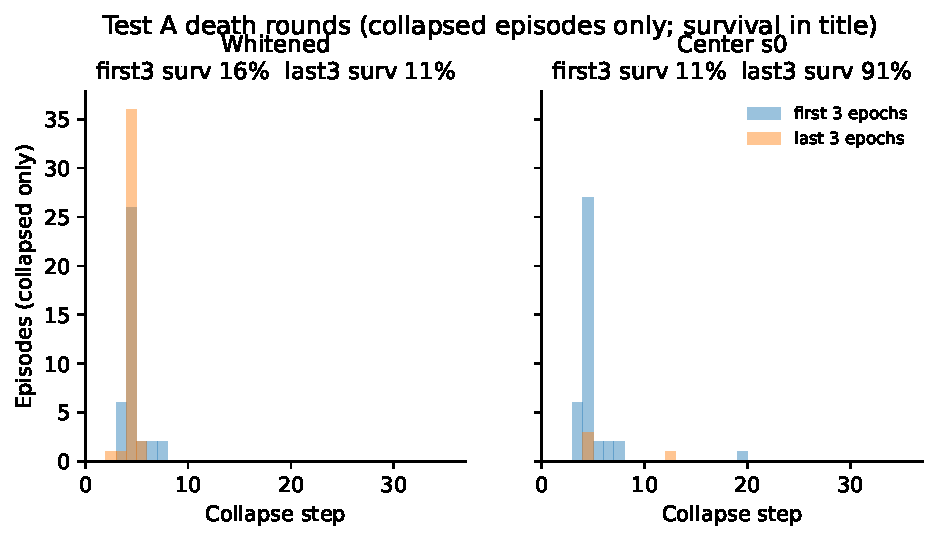
\includegraphics[width=0.92\textwidth]{figures/fig_death_rounds_testA.pdf}
\caption{Collapse step among episodes that die, first three versus last
  three epochs of Test~A.
  Pre-fix family: the whitened panel is MPS seed~0, which keeps dying
  near round~4.
  Centre-only seed~0 last epochs mostly survive (survival in the panel
  titles).
  Supporting statistic only; the claim is the opening share in
  Figure~\ref{fig:openingsA}.}
\label{fig:deathsA}
\end{figure}

The live-step mix at epoch 15 is still mostly 2s under centre (take-1
\(9\%\) on seed~0).
After open-1 that is the \(R=9\) farm.
After open-0 it is a different stock path.

\subsection{Test B --- frozen dove (always 1)}

There is no opening basin.
Open 1 and open 2 receive the same star.

\textbf{Whitened B.}
Survival \(219/225\).
Mix moved \(80\%\to 38\%\) take-2 and \(18\%\to 62\%\) take-3.
The learner farmed the dove, then smash-harvested.
It did not copy 1 (take-1 stayed in the noise).

\textbf{Centre-only B.}
Survival \(223/225\).
Live mix at the recorded readout: take-2 \(98\%\) (\(n=540\)); take-3
\(2\%\).
Open-1 share stuck at \(13\%\).
The same star sat on open 1 and open 2 (centred about \(+20\) and \(+22\)).

\textbf{Claim.}
Unflattening does not invent restraint.
Against a dove it suppresses unnecessary smash and leaves the chicken
grab: learner 2, partner 1, payoff 72, pool lives.
Whitened greed got louder (\(2\to 3\)).
Centred greed got cleaner (stay on 2).
Neither is a shaping result.

\subsection{What these robots do not license}

A frozen hawk is not two learning agents.
Centre-only Test~A does not imply that a shaper works.
The load-bearing link is narrower.
If, under the TRL default, the prior never left opening 2 even against a
partner already frozen on 2, then a two-learner table in which agent~1
opens 1 and agent~2 opens 2 could not be read as ``the shaper taught
restraint'': leave-2 would not yet be a behaviour the naive update can
produce on this budget.
The shaping grid is therefore on mean-centring, the operator that left
opening 2 by epoch 8 on three independent seeds, rather than on whitening,
which on this lock is slower and can still be mixed at epoch 15.
That choice is reported as RQ2, not as a hidden extra.

\subsection{Two learners}
\label{sec:twolearners}

Same lock, \texttt{advantage\_norm=center}, entropy 0.05.
The claim statistic remains the share of episodes that do \textbf{not}
open 2.
A 15-epoch naive table is not matched to a 50-epoch shaper table as if
they were one experiment.

\textbf{Centred naive--naive, 15 epochs, seeds 0--2.}
Survival \(119\), \(98\), \(115\) out of 225.
Last-epoch openings: seed 0, agent 1 opened 0 on all 15 games and agent 2
opened 2 on \(12/15\); seed 1, agent 1 mixed 1/2 and agent 2 opened 1 on
\(14/15\); seed 2, agent 2 opened 1 on \(13/15\).
Leave-2 in the last three epochs swapped who doves
(Table~\ref{tab:nn}, Figure~\ref{fig:whodoves}).

\textbf{Centred naive--shaper, \(3\times 15\).}
Agent 1 naive (episode update, LR \(1.41\times 10^{-6}\)).
Agent 2 shaper (trial update, LR \(3\times 10^{-7}\),
\texttt{cliprange=0.1}, \texttt{transmit\_info=true}).
Survival \(113\), \(120\), \(100\) out of 225.
Last-epoch: agent 1 left 2 on every seed (mostly 1; seed 2 mixed 0 and 1);
agent 2 opened 2 on \(14/15\), \(9/15\), \(14/15\).
Leave-2 last three epochs: agent 1 \(96\%\), \(93\%\), \(87\%\);
agent 2 \(0\%\), \(7\%\), \(2\%\).
Agent 2 leave-2 over the whole run: \(5\%\), \(5\%\), \(4\%\).
Who leaves 2 did \textbf{not} swap.

\textbf{Shaper 50 epochs, seed 0.}
Compare to 15-epoch naive \textbf{at epoch 15 only}, and to the matched
long naive below.
Epoch 1: \(2/15\) survived, both mostly opened 2.
Epoch 15: \(13/15\), agent 1 \(13\times 1\), agent 2 \(14\times 2\).
Epoch 50: \(15/15\), agent 1 \(15\times 1\), agent 2 \(15\times 2\).
Whole-run survival \(572/750\).
Agent 2 opened 0 or 1 on \(25/750\) (\(3.3\%\)) and opened 2 on
\(696/750\).
No epoch with agent-2 leave-2 majority (peak \(3/15\) at epoch 5).
Agent 1 first majority leave-2: epoch 8.
Both left 2 in the same episode \(17/750\).

\textbf{Matched long naive, 50 epochs, seed 0.}
Same config as 15-epoch naive--naive; one seed; 50 epochs.
Epoch 1: \(4/15\), both mostly opened 2.
Epoch 15: \(12/15\), agent 1 \(12\times 1\), agent 2 \(13\times 1\).
Epoch 50: \(15/15\), both \(15\times 1\), returns \(68.9\) / \(98.1\),
joint about \(167\).
Agent 2's \(98.1\) is in the direction of the deterministic
\((1,1)\)-then-\((2,3)\) fixed point at \(R=11\) (DP \(71/106\)).
The matched shaper pair at epoch 50 opened \((1,2)\) and earned about
\(143\) (open-1-then-2 versus hawk: \(71+72\)), with the shaper on \(72\).
One seed each, so a direction: this is the only executed run in which a
learner earned above the constant chicken cells, and on the H3 return
criterion the shaper is below the naive pair.
Whole-run survival \(628/750\).
Agent 1 leave-2 whole \(605/750\); agent 2 \(623/750\).
Both left 2 in the same episode \(551/750\).
First majority leave-2: agent 1 epoch 8, agent 2 epoch 9.
Last-epoch action frequencies at \(R=8\) are 100~percent open 1 for both;
later mid-stock steps are still peaked on 2.

\textbf{Info-off shaper, \(3\times 15\).}
Same trial update and LR; \texttt{transmit\_info=false}.
Survival \(118\), \(107\), \(89\) out of 225.
Who leaves 2 still did not swap.
Agent 2 leave-2 last three epochs \(18\%\), \(22\%\), \(13\%\);
whole run \(16\%\), \(19\%\), \(16\%\) (higher than info-on \(4\)--\(5\%\),
and not \(\sim 0\)).

\begin{figure}[ht]
\centering
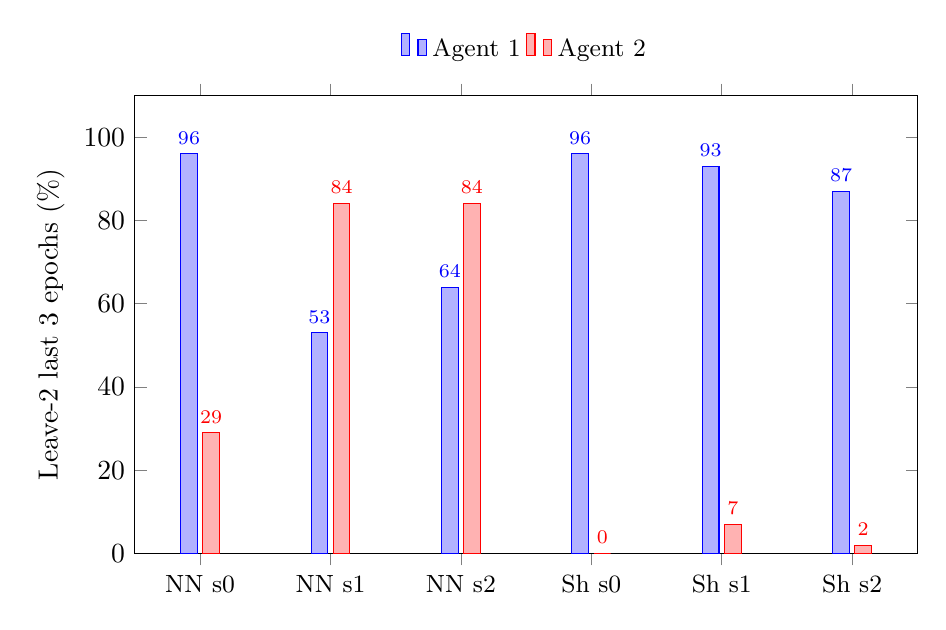
\begin{tikzpicture}
\begin{axis}[
  ybar,
  bar width=6pt,
  width=0.95\textwidth,
  height=7.4cm,
  ylabel={Leave-2 last 3 epochs (\%)},
  ymin=0, ymax=110,
  symbolic x coords={NN0, NN1, NN2, Sh0, Sh1, Sh2},
  xtick=data,
  xticklabels={NN s0, NN s1, NN s2, Sh s0, Sh s1, Sh s2},
  xticklabel style={font=\small},
  legend style={at={(0.5,1.05)}, anchor=south, legend columns=2,
    font=\small, draw=none},
  nodes near coords,
  nodes near coords style={font=\scriptsize, /pgf/number format/fixed},
]
\addplot coordinates {(NN0,96) (NN1,53) (NN2,64) (Sh0,96) (Sh1,93) (Sh2,87)};
\addplot coordinates {(NN0,29) (NN1,84) (NN2,84) (Sh0,0) (Sh1,7) (Sh2,2)};
\legend{Agent 1, Agent 2}
\end{axis}
\end{tikzpicture}
\caption{Share of episodes in the last three epochs that do not open 2.
  NN: centred naive--naive.
  Sh: centred naive--shaper with the extra trial prompt.
  Under naive--naive, which agent leaves 2 swaps across seeds.
  Under naive--shaper, agent 1 leaves 2 and agent 2 does not, on all
  three seeds.
  This figure is that contrast.
  It is not a claim that the shaper taught take-1 and then exploited.}
\label{fig:whodoves}
\end{figure}

It is not a clear shaping success.
This report does not claim that the shaper taught the naive to take 1
and then exploited by taking 2.
Who-doves did not swap under info-on or info-off; it did swap under
matched-LR naive--naive.

\textbf{Slow-LR naive--naive, \(3\times 15\).}
Both episode-update; agent 2 learning rate \(3\times 10^{-7}\).
Last epoch agent 2 opened 2 on \(12/15\) every seed.
Agent 1 leave-2 in the last three epochs: \(78\%\), \(84\%\), \(62\%\);
agent 2: \(33\%\), \(18\%\), \(27\%\).
Who-leaves-2 did not swap.
The same pattern as naive--shaper, without trial update or extra prompt.

Last-epoch returns under naive--naive seed 0 are \(70.7\) and \(75.3\),
near the \(71/72\) open-then-2 split, not the dynamic-program joint
\(210\).
No stock-conditioned 0-then-3 policy appears in last-epoch action
frequencies by stock.

\begin{itemize}
\item \textbf{Grid success (still the bar).}
  The shaper changes the opening distribution or the outcome bins
  relative to centred naive--naive, in a way that tracks the learner's
  current behaviour.
\item \textbf{Grid null.}
  Same openings, same collapse, same bins as the control.
  Live-mix will not rescue a null.
\item \textbf{Not the two-phase claim.}
  Agent 2 leave-2 on the 50-epoch seed was \(25/750\).
  Epoch 1 the shaper opened 2 while the naive still mostly opened 2.
\end{itemize}

\subsection{Noise arm (Stage B)}

Multiplicative \(\xi\in\{0.7,1.0,1.3\}\) on the growth increment.
Numbers below are reported against Table~\ref{tab:noise-dp}.

Pre-fix Test~A \(\xi\) and NN \(\xi\) were not repeated after the
trainer reseed; those two paragraphs are the shared-stream packet.
H3 is given first as that pre-fix family, then as the seed-fixed replica
(NS and slow2).

\textbf{H1--H2, Test~A + \(\xi\) (pre-fix).}
Last-epoch leave-2 is \(98\%\), \(64\%\), \(98\%\)
(openings \(15\times 0\), \(10\times 1+5\times 2\), \(15\times 0\)).
Whole-run survival \(119\), \(41\), \(93\) out of 225; last-epoch
returns \(65.5\), \(26.9\), \(58.3\).
Stage~A centre last openings were \(13\times 1\), \(14\times 1\),
\(14\times 0\).
Against a hawk, opening 0 lands in \(\{9,11,12\}\) and opening 1 in
\(\{8,9,10\}\); constant take-2 thereafter survives with probability
\(0.80\) (return \(58.3\)) from the first set and \(0.40\) (return
\(34.7\)) from the second.
Seeds 0 and 2 moved to the opening that doubles survival, which is also
the sign of \(Q(0)>Q(1)\) under noise.
Their last-epoch returns sit near that \(58.3\) cell; the mixed seed sits
nearer \(34.7\).
Leave-2 at \(R<12\) in the last epoch is \(41\%\), \(28\%\), \(29\%\),
against \(1.00\) for the feedback rule and far below its return \(68.8\).
H1 holds in a stronger form than a mere leave-2 match with Stage~A: two
of three seeds chose the DP-better exit.
H2 is negative: the learner did not learn to condition on stock.

\textbf{Naive--naive + \(\xi\) (pre-fix).}
Survival \(100\), \(43\), \(82\) out of 225; last-epoch returns
\(37.6/45.1\), \(27.9/31.1\), \(48.3/43.8\).
Seed~2 last epoch: agent 1 \(14\times 2\), agent 2 \(13\times 1\)
(leave-2 last3 \(24\%\) / \(87\%\)).
Seed~1 both still mostly opened 2 (survival \(43/225\)), where all three
Stage~A naive--naive seeds had left 2.

\textbf{H3, naive--shaper versus slow2, pre-fix.}
On the shared stream, naive--shaper survival \(90\), \(71\), \(75\) out
of 225; slow2 \(53\), \(44\), \(39\).
Agent 1 leave-2 last3: \(96\%\), \(93\%\), \(89\%\) against the shaper
versus \(69\%\), \(67\%\), \(40\%\) against slow2.
Agent 2 leave-2 last3: \(0\%\), \(11\%\), \(11\%\) (shaper) versus
\(18\%\), \(18\%\), \(20\%\) (slow2).
A more stationary hawk produced a more reliable dove on all three
\emph{nominal} paired seeds.
That agreement is one observation counted three times.

\textbf{H3, seed-fixed, same noise-table pairing, all L40S.}
Seed 0 of each arm is the pre-fix seed-0 tape (opening identity \(1.00\)).
Seeds 1 and 2 are new.
Naive--shaper last3 survival \(36/45\), \(12/45\), \(5/45\); last-epoch
return \(49.7\), \(29.0\), \(12.3\); agent-1 leave-2 last3 \(96\%\),
\(44\%\), \(33\%\); agent-2 leave-2 last3 \(0\%\), \(22\%\), \(22\%\).
Slow2 last3 survival \(21/45\), \(24/45\), \(8/45\); last-epoch return
\(44.8\), \(52.9\), \(13.0\); agent-1 leave-2 last3 \(69\%\), \(76\%\),
\(27\%\); agent-2 leave-2 last3 \(18\%\), \(13\%\), \(22\%\).
Sign of NS minus slow2 on agent-1 leave-2 last3 is \(+\), \(-\), \(+\);
on last-epoch return \(+\), \(-\), \(-\).
Both agent 2s stay mostly on 2.
Learning rate and clip are matched; the remaining difference is the
trial update and the extra prompt.
The 36-unit DP interest in feedback restraint was not collected
(seed-fixed NS leave-2 at \(R<12\) is \(51\%\), \(18\%\), \(27\%\)
for the naive and \(2\%\), \(12\%\), \(5\%\) for the shaper; returns sit
near hawk--dove or collapse, not \(72/68.8\)).
H3 as a shaper-return and more-reliable-dove inequality fails at three
independent seeds.
The pre-fix ``more reliable dove on all three seeds'' does not survive
the replica.
A 50-epoch slow2 \(\xi\) seed 0 continues the 15-epoch snapshot: first
agent-1 majority at epoch 10, last-open \(15\times 0\) versus mixed
agent 2, last-epoch return \(70.5/69.2\), last3 survival \(37/45\).
NS \(\xi\) at 50 epochs was not obtained.

\section{Final grid}
\label{sec:grid-results}

The tables and figures in this section are written by
\texttt{scripts/evaluate\_grid.py} from the records of the final grid
(Chapter~\ref{ch:design}); where a file is absent the arm has not been
run.
\newcommand{\gridinput}[1]{\IfFileExists{tables/grid/#1}{\input{tables/grid/#1}}{\emph{[not yet run: }\texttt{\detokenize{#1}}\emph{]}}}

\subsection{Checks C1 and C2}
\gridinput{B_c2.tex}

\subsection{Stage A: H-A}
\begin{table}[ht]\centering\small
\caption{Stage~A, last-window estimates per arm and seed (interval: Wilson 95\%; return: mean and standard error over the window's games).}
\label{tab:grid-A-arms}
\resizebox{\textwidth}{!}{\gridinput{A_arms.tex}}
\end{table}
\begin{table}[ht]\centering\small
\caption{Stage~A, paired ladder differences \(\Delta_s\) with sign agreement over seeds.}
\label{tab:grid-A-rungs}
\resizebox{\textwidth}{!}{\gridinput{A_rungs.tex}}
\end{table}

\subsection{Stage B: the ladder, H-B1 to H-B4}
\begin{table}[ht]\centering\small
\caption{Stage~B, last-window estimates per arm and seed.}
\label{tab:grid-B-arms}
\resizebox{\textwidth}{!}{\gridinput{B_arms.tex}}
\end{table}
\begin{table}[ht]\centering\small
\caption{Stage~B, paired ladder differences \(\Delta_s\) with sign agreement over seeds.}
\label{tab:grid-B-rungs}
\resizebox{\textwidth}{!}{\gridinput{B_rungs.tex}}
\end{table}
\begin{figure}[ht]\centering
\IfFileExists{figures/grid/B_curves.pdf}{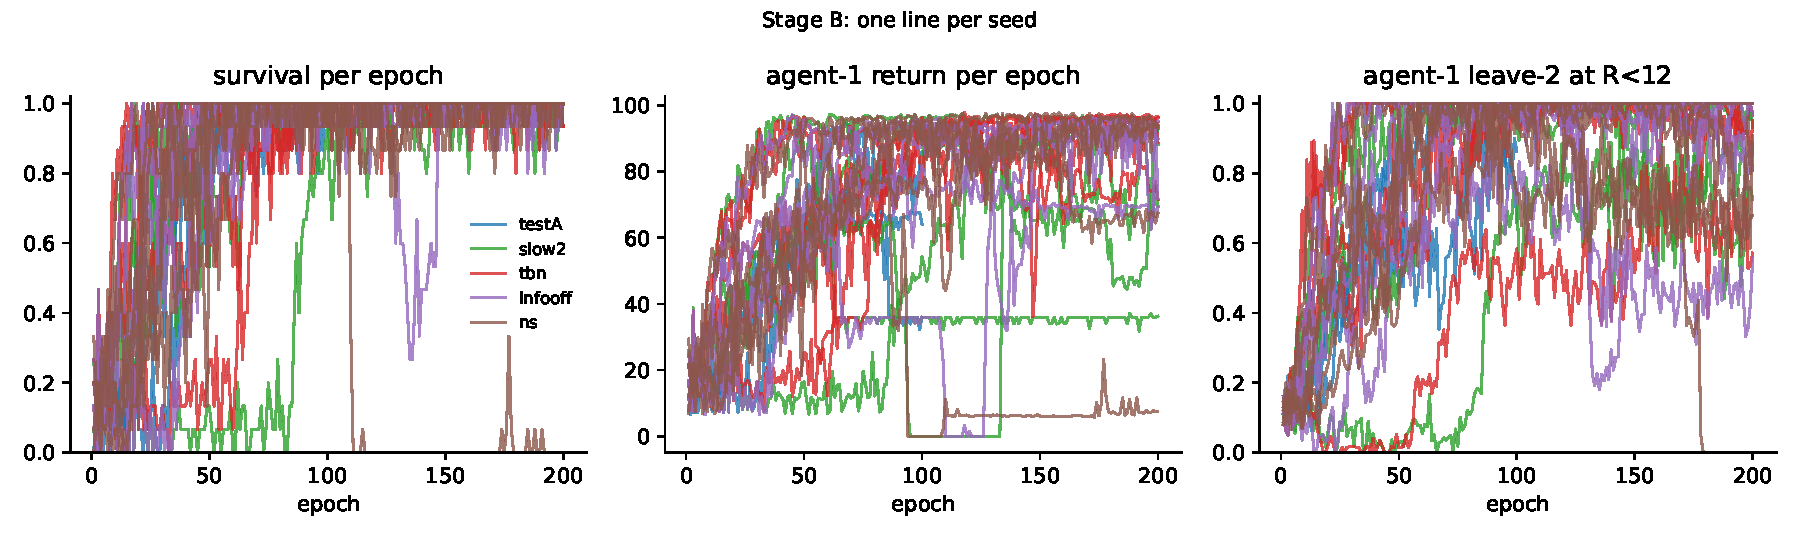
\includegraphics[width=\textwidth]{figures/grid/B_curves.pdf}}{\emph{[not yet run: B\_curves.pdf]}}
\caption{Stage~B learning curves: survival, agent-1 return and agent-1 low-stock restraint per epoch, one line per seed, colour per arm.}
\label{fig:grid-B-curves}
\end{figure}

\subsection{Transfer: H-T}
\gridinput{B_transfer.tex}

\subsection{Sensitivity}
\gridinput{sensitivity.tex}
